\documentclass[a4paper,12pt]{report}
\usepackage[utf8]{inputenc}
\usepackage{amsmath}
\usepackage{graphicx}
\usepackage{listings}
\usepackage{tikz}
\usepackage[T1]{fontenc}
\usepackage{color}
\usetikzlibrary{arrows,automata}
\DeclareUnicodeCharacter{00A0}{~}
\definecolor{pythonred}{rgb}{0.6,0,0} % for strings
\definecolor{pythongreen}{rgb}{0.25,0.5,0.35} % comments
\definecolor{pythonpurple}{rgb}{0.5,0,0.35} % keywords
	\definecolor{pythondocblue}{rgb}{0.25,0.35,0.75} % javadoc
	\renewcommand{\thechapter}{}
	\renewcommand{\chaptername}{}
	\lstset{language=python,
	basicstyle=\ttfamily,
	keywordstyle=\color{pythonpurple}\bfseries,
	stringstyle=\color{pythonred},
	commentstyle=\color{pythongreen},
	morecomment=[s][\color{pythondocblue}]{/**}{*/},
	numbers=left,
	numberstyle=\tiny\color{black},
        stepnumber=2,
	numbersep=10pt,
	tabsize=4,
	showspaces=false,
	showstringspaces=false}

% Title Page

 \title{\bfseries\huge \textcolor{red}{\underline {EEP-702 Network Lab}} \\{\textcolor{blue}{Assignment1-Simulating a Network Topology in NS2:}}}
\author{\bfseries\large\textcolor{black} {Harshit Kumar Gupta}\\ {\textcolor{black}{2013EET2369}}\\

\includegraphics[width=3cm,height=3.4cm]{./iit.png}\\\noindent Computer Technology\\
\noindent Department Of Electrical Engineering\\IIT DELHI}
% iit.png: 282x282 pixel, 72dpi, 9.95x9.95 cm, bb=0 0 282 282
\begin{document}
\maketitle
\tableofcontents


\chapter{\textcolor{blue}{\underline {PROBLEM STATEMENT}}}
\noindent 
         Working onn the Network Simulator to :
	
	\begin{enumerate}
	  \item Simulating a network topology in.
	  \item Effect of bottleneck nodes.
 
	\end{enumerate}

Consider the topology as shown below where T1...T6  are transmitters and R1....R6 are receivers.
 R1 receives from T1, R2 receives from T2 and so on. B1,B2 and B3 act as bottleneck nodes
 and also provide for routing of packets. Consider queuing systems as RED for B1,SFQ for B2
  and FIFO for B3.

\begin{center}
\chapter{\textcolor{blue}{\underline {ABSTRACT}}}
\end{center}
\noindent The entire code has been written as to simulate on a Network Simulator which inputs a 'tcl' file and when compiled with a ns2 Simulator generates a 'trace' and 'nam' file as Output.
	  Furthermore awk tool has been used as to extract the columns of the trace file and to act them as parameters for deciding the effect of bottlenecks in the Network through
	  realising the Packet Size and the inter delay time between the packets. Finally the value of those parameters is plotted using the 'gnuplot' tool so as to get the  values through a graph.


\begin{center}
\chapter{\textcolor{blue}{\underline {INTRODUCTION}}}
\end{center}
\noindent \textbf In 1996-97, ns version 2 (ns-2) was initiated based on a refactoring by Steve McCanne. Use of Tcl was replaced by MIT's Object Tcl (OTcl), an object-oriented dialect of Tcl.
		  The core of ns-2 is also written in C++, but the C++ simulation objects are linked to shadow objects in OTcl and variables can be linked between both language realms.
		  Simulation scripts are written in the OTcl language, an extension of the Tcl scripting language.
                  Presently, ns-2 consists of over 300,000 lines of source code, and there is probably a comparable amount of contributed code that is not integrated directly into the main distribution of ns-2 exist,
                  both maintained and unmaintained. It runs on GNU/Linux, FreeBSD, Solaris, and Mac OS X.
		  \\AWK is an interpreted programming language designed for text processing and typically used as a data extraction and reporting tool. 
		  It is a standard feature of most Unix-like operating systems. AWK was very popular in the late 1970s and 1980s, but from the 1990s has largely been replaced by Perl,
		  on which AWK had a strong influence.
		  
		 While the gnuplot is a command-line program that can generate two- and three-dimensional plots of functions, data, and data fits. 
		    It is frequently used for publication-quality graphics as well as education.gnuplot can produce output directly on screen, 
		    or in many formats of graphics files, including Portable Network Graphics (PNG), Encapsulated PostScript (EPS), Scalable Vector Graphics (SVG), JPEG and many others. 
		    It is also capable of producing LaTeX code that can be included directly in LaTeX documents, making use of LaTeX's fonts and powerful formula notation abilities.
		    The program can be used both interactively and in batch mode using scripts.

\begin{center}
\chapter{\textcolor{blue}{\underline {SPECIFICATIONS AND ASSUMPTIONS}}}
\end{center}
\section*{Specifications}
\begin{enumerate}
 
 \item Queue length of B1 = 1000
 \item Queue length of B2 = 1000 
\item Queue length of B3 = 2000
 \item Bandwidth of Ti-Bi links = 200 kbps
 \item Bandwidth of B1-B3 link  500 kbps
 \item Bandwidth of  B2-B3 link = 500 kbps 
\item Bandwidth of B3-Ri links = 200 kbps

\end{enumerate}

\section*{Assumptions}
\begin{enumerate}
\item ns2 Simulator will be used for compiling the tcl file.
\item Inspite of perl ; 'awk' tool will be used to cut the parameters.
\item 'gnuplot' has been used to plot the values to study bottlenecks.
\item Other throughput degradation factors have been ignored.
\end{enumerate}
 
\begin{center}
\chapter{\textcolor{blue}{\underline {METHODOLOGY}}}
\end{center}
The methodology that is used for developing this project work is defined below:
\begin{enumerate} 
\item The entire code is written in tcl file format.
\item First of all all the required 15 nodes are created. Out of which 6 are sender and 6 are receiver nodes.
\item Of them 3 nodes act as Routers which transmit packet from sender to Receiver.
\item Links are Duplex and are created as per Specifications above.
\item A FTP  traffic source is Setup over the TCP agent.
\item Once the file is compiled it , the Output trace file is generated.
\item nam file is used for simulation of network in given topology.
\item trace file is used for analyis of network
\end{enumerate}

\begin{center}
\chapter{\textcolor{blue}{\underline {Execution Directive}}}
\end{center}
The Directions to how do we execute the program as to accomplish the project.
\begin{enumerate} 
\item Reach the Path of the Project Folder using cd assign1
\item Compile the tcl file by  ns tcl-script.tcl [parameters]  
\item trace-output.tr and nam-output.nam file is genearted.
\item Cut the Parameter columns using awk as   awk -f filename.awk filename.tr >parameters.dat 
\item plot the parameters using the gnuplot as  Write gnuplot on Terminal 
\item gnuplot throughput.plot ;gnuplot interarrival.plot
\item This us how we get the graphical analysis of our network.

\end{enumerate}



\begin{center}
\chapter{\textcolor{blue}{\underline {Simulation}}}


 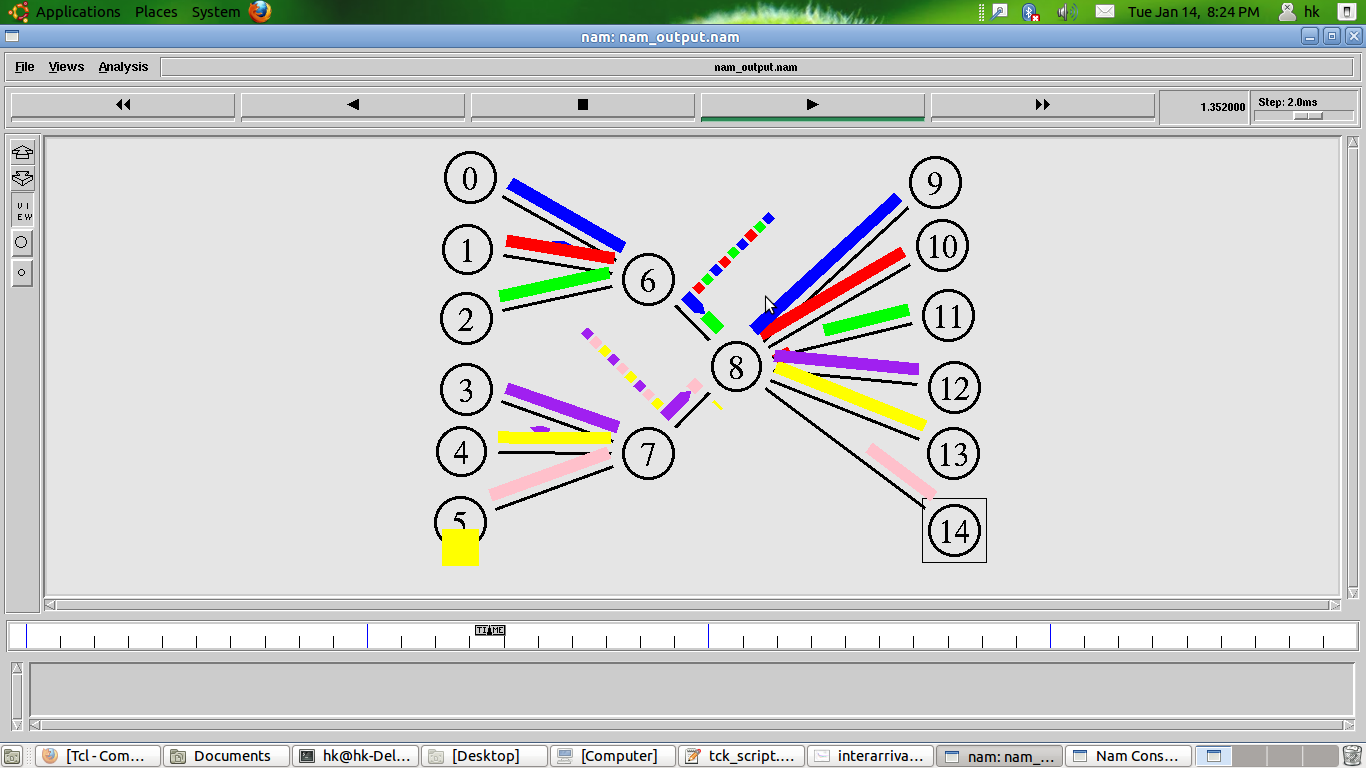
\includegraphics[width=13 cm,height=13 cm]{./simulation.png}
 % flowchart.png: 668x744 pixel, 72dpi, 23.57x26.25 cm, bb=0 0 668 744


\end{center}

\begin{center}
\chapter{\textcolor{blue}{\underline {OUTPUT GRAPH}}}

 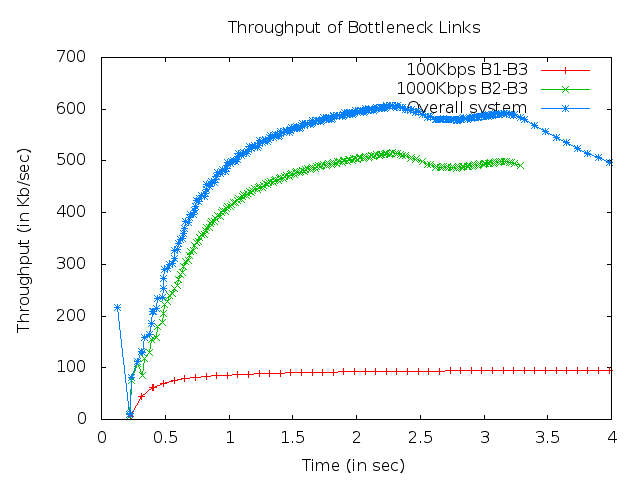
\includegraphics[width=15 cm,height=15 cm]{./link_throughput.png}
 
Throughput Analysis of links
\end{center}
\begin{center}
 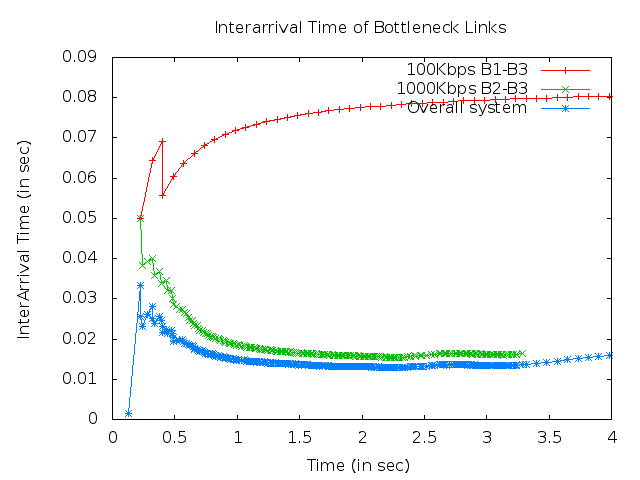
\includegraphics[width=15 cm,height=18cm]{./link_interarrival.png}

InterArrival Delay Analysis of links
\end{center}
\begin{center}
 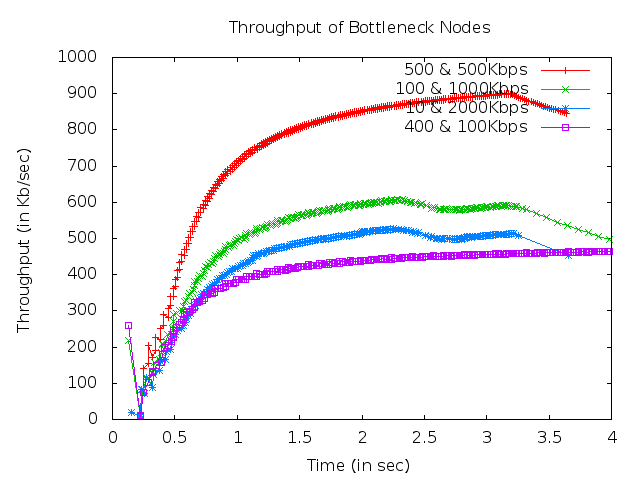
\includegraphics[width=15 cm,height=18 cm]{./throughput.png}

Throughput Analysis of network topology
\end{center}

\begin{center}
 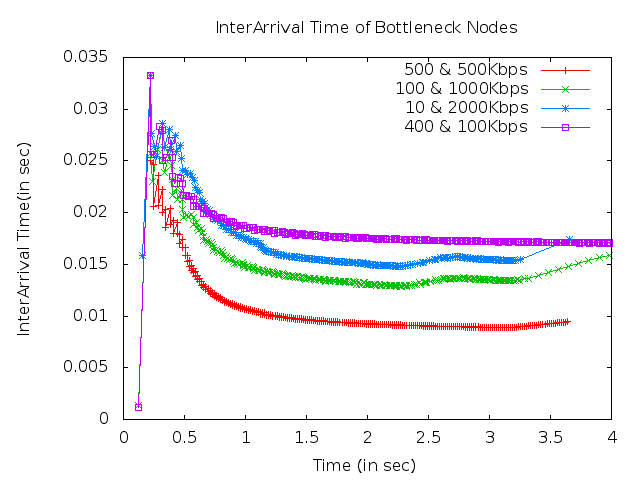
\includegraphics[width=15 cm,height=18 cm]{./interarrival.png}

InterArrival Time Analysis of network topology
\end{center}





\begin{center}
\chapter{\textcolor{blue}{\underline {RESULTS AND CONCLUSIONS}}}
\begin{enumerate}
\item For FTP traffic analysis over TCP client .tr(trace) file is used.
\item We used 'awk' utility to know performance parameters in network by extracting data from trace file.
\item For simulation of network .nam(network animator file)is used which gives proper visualization of transfer of packets and loss of packets in network topology. 
\item Finally we use gnuplot to show the Graph of throughput and inter arrival time.
\item  Plotted graphs show  differnt  behaviour of Network under differnt Bandwidth of bottleneck links.
\item Throughput and InterArrival Packet Delay of whole system depends on bandwidth of faster bottleneck link.On increasing Bandwidth throughput increases and InterArrival Delay decreases.

\end{enumerate}
\end{center}
\end{document}  